\documentclass[UTF8]{beamer}
\usepackage[utf8]{inputenc}
\usepackage{ctex}
\usefonttheme[onlymath]{serif}
\usetheme{Madrid}
\usecolortheme{default}

%------------------------------------------------------------
%This block of code defines the information to appear in the
%Title page
\title{Exact Algorithms of Graph Coloring}
\author{\heiti 231240058  陈小川}
\institute{Nanjing University}
\date{\heiti 2024 年 12 月 5 日}

% 自定义颜色
\definecolor{customgreen}{RGB}{0,96,0} % 深绿色
\definecolor{lightgreen}{RGB}{230,239,230} % 浅绿色背景

% 自定义绿色方框环境
\newenvironment{customexample}[1]{%
  \setbeamercolor{block title}{fg=white,bg=customgreen}%
  \setbeamercolor{block body}{fg=black,bg=lightgreen}%
  \begin{block}{#1}}{\end{block}}

%End of title page configuration block
%------------------------------------------------------------



%------------------------------------------------------------
%The next block of commands puts the table of contents at the 
%beginning of each section and highlights the current section:

\AtBeginSection[]
{
  \begin{frame}
    \frametitle{Table of Contents}
    \tableofcontents[currentsection]
  \end{frame}
}
%------------------------------------------------------------


\begin{document}

%The next statement creates the title page.
\frame{\titlepage}


%---------------------------------------------------------
%This block of code is for the table of contents after
%the title page
\begin{frame}
\frametitle{Table of Contents}
\tableofcontents
\end{frame}
%---------------------------------------------------------


\section{二分图边染色}

%---------------------------------------------------------
%Changing visivility of the text
\begin{frame}
  \frametitle{\text{\heiti 动机}}
\begin{figure}
  \centering
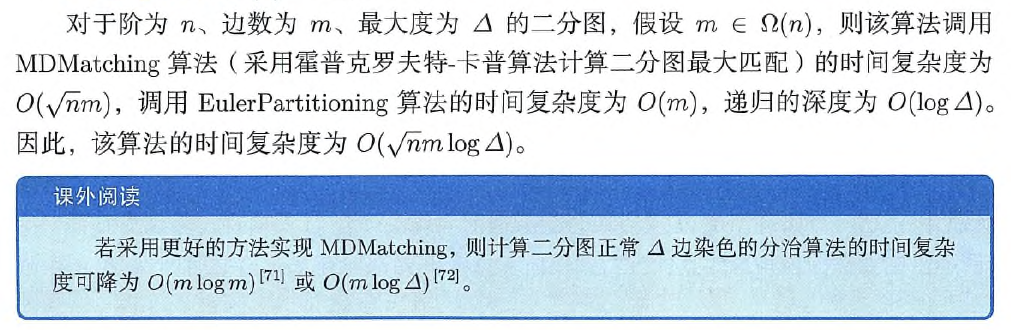
\includegraphics[scale=0.4]{figs/motivation.png}
\end{figure}
\pause
\begin{itemize}
  \item \text{\heiti 如何在 $O(m \log m)$ 时间内找出二分图的正常 $\Delta$ 边染色?}
\end{itemize}
\end{frame}

\begin{frame}
  \frametitle{\text{\heiti 算法回顾}}
  对二分图的最大度分类讨论
  \begin{itemize}
    \item 若最大度为偶数,则将原图拆分成两个子图使得每个子图最大度等于原来的一半
    \item 若最大度为奇数,则找出原图一个饱和所有度数等于最大度的顶点的匹配,将其染成同一种颜色并删去,于是就能归结为偶数的情形
  \end{itemize}
\end{frame}

\begin{frame}
\frametitle{改进思路}
\begin{itemize}
  \item 将二分图转化为正则二分图
  \item 对正则二分图进行分治染色
\end{itemize}
\end{frame}

%---------------------------------------------------------


%---------------------------------------------------------
%Example of the \pause command
\begin{frame}
  \frametitle{转正则二分图}
  对于二分图 $G = \langle L \cup R, E \rangle$
  \begin{itemize}
    \item 若存在 $u, v \in L$,使得 $d(u) + d(v) \leq \Delta$,则将 $u$ 和 $v$ 合并为一个点,重复操作直至不存在这样的 $u, v$
    \item 对于 $R$ 同理
    \item 如果合并后两边点的数目不等,则在点数较少的那边补足,记两侧点集为 $L', R'$
    \item 若存在 $u \in L'$,$d(u) < \Delta$,则必存在 $v \in R'$,$d(v) < \Delta$,在图上新加一条边 $u v$,重复操作直至图为正则二分图
  \end{itemize}
\end{frame}

\begin{frame}
  \frametitle{转正则二分图}
  \begin{block}{Lemma}
    在进行上述操作后,图的边数至多为 $2m + \Delta$
  \end{block}
  \begin{block}{证}
    不妨假设合并后 $|L| \geq |R|$,至多有一个顶点 $v_0$ 满足 $d(v_0) \leq \frac{\Delta}{2}$,因此
    添加的边数为,
    \[\begin{aligned}
      \sum_{v\in L} \Delta - d(v) &\leq \sum_{v \in L} [2d(v) - d(v)] + \Delta\\
      &=m+\Delta
    \end{aligned}\]
    因此转为二分图后边数仍然为 $O(m)$
  \end{block}
\end{frame}

\begin{frame}
  \frametitle{欧拉划分}

  假设图是正则二分图且每个顶点度数均为偶数,欧拉划分将会更简单:
  \begin{itemize}
    \item 只需要对图的每个连通分支找出一条欧拉回路,然后交替地把边放到两个子图当中
  \end{itemize}

\end{frame}

\begin{frame}
  \frametitle{完美匹配}

  \begin{block}{定理}
    任何非空 $k$ 正则二分图均有完美匹配
  \end{block}

  \begin{block}{证}
    利用霍尔定理即可
  \end{block}
\end{frame}

\begin{frame}
  
  \frametitle{完美匹配}
  \textbf{$O(m \log m)$ 时间求完美匹配}
  \begin{itemize}
    \item 取最小的 $t$ 使得 $2^t \geq m$,令 $\alpha = \lfloor \frac{2^t}{k} \rfloor, \beta = 2^t - k \alpha$,将图中每条边复制为 $\alpha$ 条重边,再将 $L$ 和 $R$ 中的点两两配对(不一定要有边),每对点之间添加 $\beta$ 条虚拟边,最后得到 $2^t$ 正则图
    \item 对这个图做欧拉划分,得到 $2^{t-1}$ 正则子图 $H_1$ 和 $H_2$,选择 $H_1$ 和 $H_2$ 中虚拟边较少的再次做欧拉划分,重复 $t$ 次就能得到完美匹配
  \end{itemize}

\end{frame}


\begin{frame}
  \frametitle{完美匹配}
  \textbf{如何在 $O(m)$ 时间内完成欧拉划分}
  % \begin{center}
  %   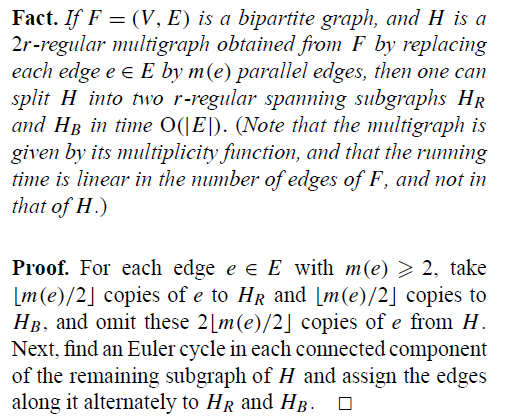
\includegraphics[scale=0.6]{figs/algo.png}
  % \end{center}
  \begin{itemize}
    \item 我们注意到前面的 $2^t$ 正则图边数比原来多了很多,
    但有很多重边,经过去重的边数是 $O(m)$ 的
    \item 对于边 $e$,假设他有 $m(e)$ 条重边,我们将其中 $\lfloor \frac{m(e)}{2} \rfloor$ 条放入一个子图 $H_R$,
    另外 $\lfloor \frac{m(e)}{2} \rfloor$ 放入另一个子图 $H_B$ 
    \item 对于每条边都如此操作,最后每条边都只剩下 1 或 0 条重边,边数为 $O(m)$,再在这张图上跑欧拉划分就是 $O(m)$ 的
  \end{itemize}
\end{frame}

\begin{frame}
  \frametitle{完美匹配}

  \begin{block}{Theorem}
    上述过程得到的是原图的完美匹配
  \end{block}


  \begin{block}{证}
    只需证明两件事
    \begin{itemize}
      \item 得到的是 $2^t$ 正则图的完美匹配
      \\重复操作 $t$ 轮后得到的是 $1$ 正则图,因此正好是 $2^t$ 正则图的完美匹配
      \item 结果不包含虚拟边
      \\ 虚拟边的数量为 $\beta n < k n = m \leq 2^t $,经过 $t$ 轮以后就全部被筛掉了
    \end{itemize}
  \end{block}

\end{frame}

\begin{frame}
  \frametitle{分治染色}
  仍对图的最大度分奇偶讨论
  \begin{itemize}
    \item 如果最大度为偶数,我们可以在 $O(m)$ 时间内完成欧拉划分,将问题归结为对两个子图的染色
    \item 如果最大度为奇数,我们可以在 $O(m \log m)$ 时间内找出完美匹配并将其删去
  \end{itemize}
  \pause
  \begin{block}{时间复杂度分析}
    若度数 $k$ 为偶数,有
    \[T(m) = 2 T(m / 2) + O(m)\]
    若 $k$ 为奇数,有
    \[T(m) = 2 T(m / 2) + O(m \log m)\]
    利用主定理即可得到 $T(m) = O(m \log m)$
  \end{block}
\end{frame}

%---------------------------------------------------------

\section{一般图点染色}

%---------------------------------------------------------
%Highlighting text

\begin{frame}
  \frametitle{整数规划}
  \begin{customexample}{Definition}
    对于图 $G = \langle V, E \rangle$ 定义两个 0-1 矩阵 $\bold{X}_{n \times n}$ 和 $\bold{Y}_{n}$,含义如下:
    \[X_{ij} = \begin{cases}
      1 \text{ if vertex } v_i \text{ is assigned to color } j,\\
      0 \text{ otherwise}
    \end{cases}\]
    \[Y_{j} = \begin{cases}
      1 \text{ if at least one vertex is assigned to color }j,\\
      0 \text{ otherwise}
    \end{cases}\]
  \end{customexample}
  \textbf{约束条件}
  \[X_{ij} + X_{lj} \leq Y_j \quad \forall (v_i, v_l) \in E, \forall j \in \{1, \dots, n\}\]
  \[\sum_{j = i}^{n} X_{i j} = 1 \quad \forall v_i \in V\]
  \[X_{ij}, Y_j \in \{0, 1\}\]
\end{frame}

\begin{frame}
  \frametitle{例子}
  \begin{customexample}{Example}
    \begin{columns}
      \column{0.5\textwidth}
      \[
      \bold{X} = \begin{pmatrix}
        0 & 0 & 0 & 1\\
        1 & 0 & 0 & 0\\
        0 & 0 & 1 & 0\\
        0 & 0 & 0 & 1\\
      \end{pmatrix}\]
      \[
      \bold{Y} = \begin{pmatrix}
        1 & 0 & 1 & 1
      \end{pmatrix}
      \]
      \column{0.5\textwidth}
      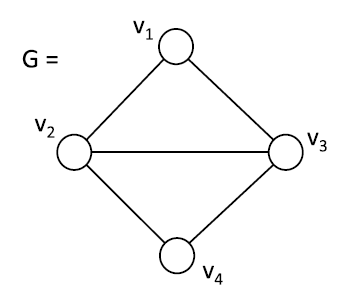
\includegraphics[scale=0.5]{figs/exp2.png}
    \end{columns}
  \end{customexample}
\end{frame}

\begin{frame}
  \frametitle{分支定界法}
    \begin{columns}
      \column{0.4\textwidth}
      \begin{itemize}
        \item 先去除整数约束,即把每个变量都当成 $[0, 1]$ 区间上的连续变量,就相当于求解一次线性规划
        \item 如果线性规划的解为整数解,那么就是最优解
        \item 如果不是整数解,任取解中非整数的一个变量 $X_{ij}$,分两种情况,将 $X_{ij}$ 的取值加入约束条件递归求解
        \begin{itemize}
          \item $X_{ij} = 0$
          \item $X_{ij} = 1$
        \end{itemize}
      \end{itemize}
      \column{0.6\textwidth}
      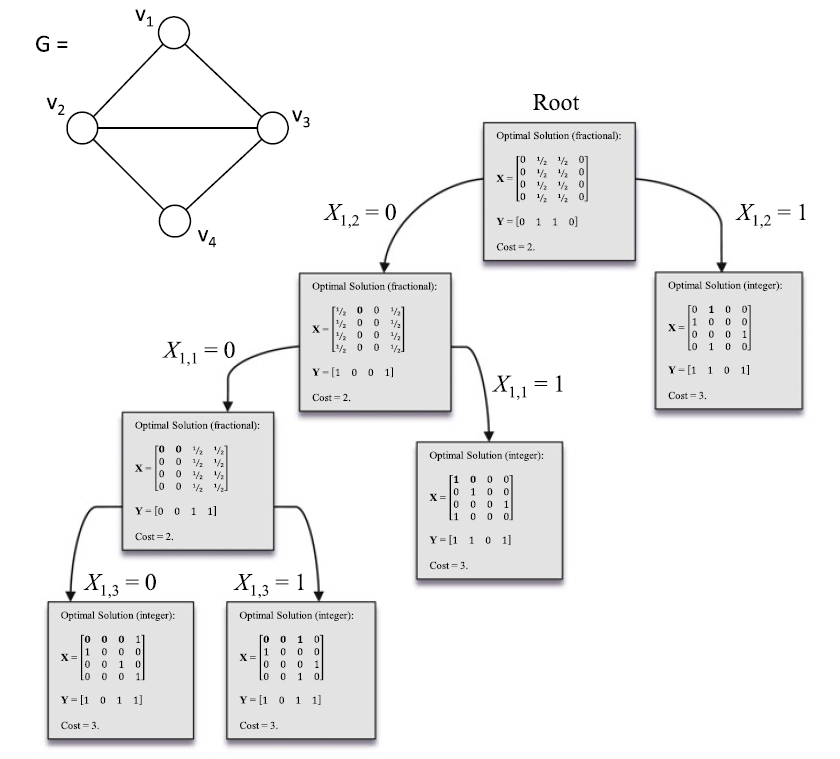
\includegraphics[scale=0.33]{figs/branch-bound.png}
    \end{columns}
\end{frame}

\begin{frame}
  \frametitle{分支定界法}
  
  在分支定界法运行过程中,我们需要维护两个值
  \begin{itemize}
    \item 迄今为止所取得的最优整数解,如果某一节点线性规划的结果高于这一值,就不需要扩展这一节点了,可以将其标注为 fathomed
    \item 所有 unfathomed 的叶子节点的线性规划最优解,一旦有整数解到达这个界,就可以直接结束程序了
  \end{itemize}

\end{frame}

\begin{frame}
  \frametitle{模型优化}
  
  我们的模型有一个很大的缺点,就是会形成很多对称的解,例如,对 $\bold{X}$ 和 $\bold{Y}$ 的列进行重排就能得到两个表示不同但本质一样的解
  \begin{center}
    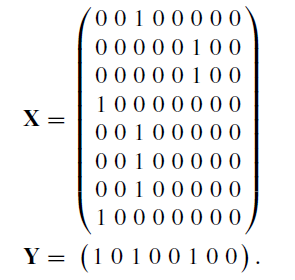
\includegraphics[scale=0.5]{figs/sol1.png}
  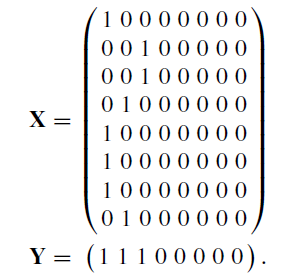
\includegraphics[scale=0.5]{figs/sol2.png}
  \end{center}
  
\end{frame}

\begin{frame}
  \frametitle{模型优化}

  解决方法是添加更多的约束,例如
  \[Y_j \geq Y_{j + 1} \quad \forall j \in \{1, \dots, n-1\}\]
  \begin{center}
    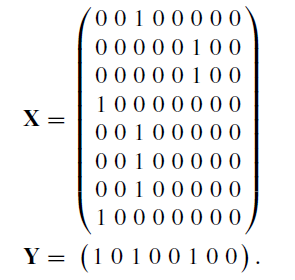
\includegraphics[scale=0.5]{figs/sol1.png}
    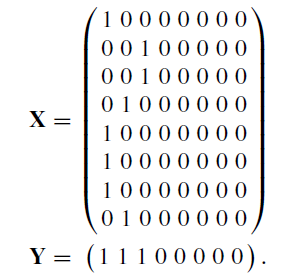
\includegraphics[scale=0.5]{figs/sol2.png}
  \end{center}
\end{frame}

\begin{frame}
  \frametitle{模型优化}

  但同一组解仍对应整数规划的 $k!$ 组解,可以进一步约束:
  \[\sum_{i = 1}^{n} X_{i j} \geq \sum_{i = 1}^{n} X_{i j + 1}, \quad \forall j \in \{1,\dots,n-1\}\] 

  \pause
  还是有可能重复,可以把前面的约束替换为下面两个约束:
  \[X_{i j} = 0 \quad \forall v_i \in V, j \in \{i + 1, \dots, n\}\]
  \[X_{i j} \leq \sum_{l = j - 1}^{i - 1} X_{lj-1} \quad \forall v_i \in V - \{v_1\}, \forall j \in \{2, \dots, i-1\}\]
  实际上就是将 $\bold{X}$ 的所有列向量按字典序进行了排序

\end{frame}

\begin{frame}
  \frametitle{模型优化}

  在这一约束下同一个解就只能有一种表示
  \begin{center}
    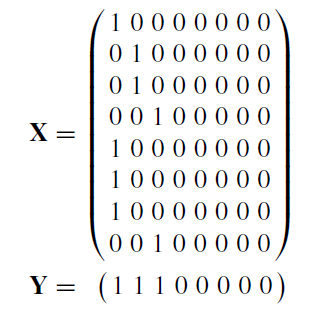
\includegraphics[scale=0.5]{figs/sol3.png}
  \end{center}
\end{frame}

\begin{frame}
  \frametitle{References}

  1. Alon, Noga (2003), "A simple algorithm for edge-coloring bipartite multigraphs", Information Processing Letters, 85 (6): 301–302, doi:10.1016/S0020-0190(02)00446-5, MR 1956451, S2CID 34965604
  
  2. R. M. R. Lewis (2021), Guide to Graph Colouring,
  Algorithms and Applications. 

\end{frame}
 
%---------------------------------------------------------


\end{document}